\documentclass[11pt]{article}

\usepackage[margin=1in]{geometry}
\usepackage{booktabs}
\usepackage{hyperref}
\usepackage{amsmath}
\usepackage{graphicx}
\usepackage{url}
\usepackage{tikz}
\usepackage{placeins}
\usetikzlibrary{arrows.meta,positioning}

\title{Contract-First Local LLM Reliability for Structured Outputs}
\author{Rana Muhammad Usman\\
\texttt{usmanashrafrana@gmail.com}}
\date{February 2026}

\begin{document}
\maketitle

\begin{abstract}
Local language models are increasingly used for tasks that require machine-readable outputs
(e.g., JSON, SQL, or code stubs), yet such outputs are often malformed or inconsistent.
We present \textit{contract-first generation}, a lightweight reliability layer that enforces
structured JSON contracts, validates outputs, optionally repairs invalid responses, and
deterministically compiles them into final artifacts (SQL or code).
On a 50-prompt structured benchmark, we evaluate contract-first on two model families.
For code-specialized models (Qwen2.5-Coder 7B), contract-first improves validity from 0.70 to 1.00,
with SQL validity improving from 0.00 to 1.00. However, for general-purpose models (Llama 3.2 3B),
contract-first can reduce validity (0.96 $\rightarrow$ 0.68) due to the added complexity of
JSON AST formats. This reveals a key tradeoff: contract-first works best when models are
already proficient at structured output. A fast/slow pairing (1.5B + 7B) achieves 0.98 validity
with lower latency. The method requires no constrained decoding, unit tests, or external
infrastructure---only standard text generation and JSON validation.
\end{abstract}

\section{Introduction}
Local LLMs offer privacy and low marginal cost, but reliability remains a barrier.
Many user tasks require outputs that are syntactically valid and machine-consumable,
yet free-form generation frequently produces malformed JSON, non-parseable SQL, or
incomplete code stubs. For most users, unit tests and evaluation infrastructure do not exist.

We study a simple and general approach: \textit{contract-first generation}. Instead of
asking a model to output the final artifact directly, we first ask for a structured JSON
representation constrained by a schema (the \emph{contract}). We validate this output and,
if needed, repair it. We then compile the structured representation into the final artifact.

This approach aims to deliver (1) higher validity rates without tests, (2) shorter outputs,
and (3) predictable behavior across models.

\section{Related Work}

\textbf{Constrained decoding.}
Several systems enforce structured outputs by constraining token sampling at decode time.
Outlines~\cite{outlines} uses finite-state machines to guarantee outputs match a JSON schema
or regular expression. Guidance~\cite{guidance} interleaves generation with programmatic
constraints. SGLang~\cite{sglang} compiles structured generation programs into efficient
execution plans. Grammar-based sampling in llama.cpp~\cite{llamacpp_grammar} restricts tokens
to those allowed by a BNF grammar. These approaches are highly effective but require
integration with the inference engine, which may not be available for all deployment scenarios.

\textbf{Post-hoc validation.}
An alternative is to validate and repair outputs after generation.
Instructor~\cite{instructor} validates LLM outputs against Pydantic schemas and retries on
failure. Jsonformer~\cite{jsonformer} guarantees JSON structure by generating only the
variable portions. OpenAI's structured outputs~\cite{openai_structured_outputs} and
LMQL~\cite{lmql} support schema-constrained generation through API features.

\textbf{Our approach.}
Contract-first generation is a post-hoc validation method designed for local models without
constrained decoding support. Unlike Instructor (which targets API-based models), we focus on
lightweight, local-first deployment. Unlike grammar-based methods, we require no inference
engine modifications---only standard text generation. We validate against JSON Schema~\cite{json_schema},
repair invalid outputs, and compile structured representations into final artifacts (SQL, code).
Our evaluation follows the spirit of verifiable-instruction benchmarks~\cite{ifeval}, focusing
on syntactic validity rather than subjective quality.

\section{Method}
\subsection{Contract-First Pipeline}
Given a user request, we apply a contract-first pipeline:
\begin{enumerate}
  \item \textbf{Contract prompt}: Request a JSON output that matches a strict schema.
  \item \textbf{Validation}: Parse the JSON and validate it against the schema.
  \item \textbf{Repair (optional)}: If invalid, request a corrected JSON output.
  \item \textbf{Compilation}: Deterministically compile JSON into the final artifact.
\end{enumerate}

\begin{figure}[h]
\centering
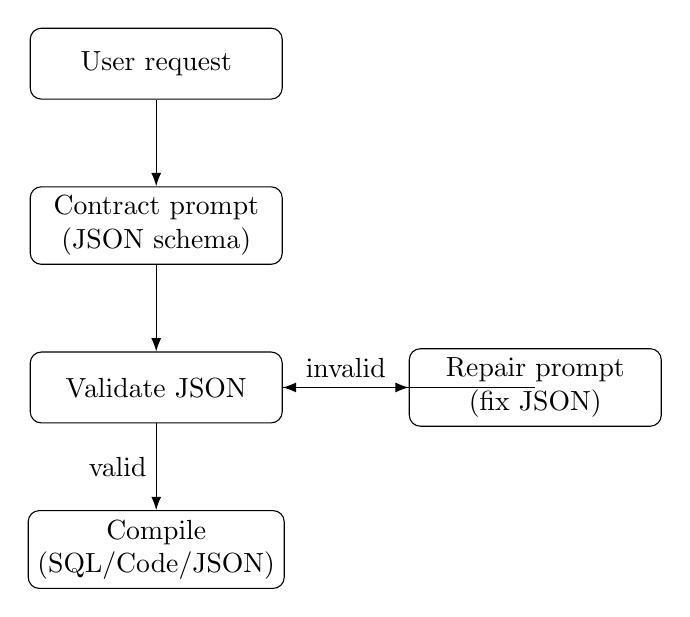
\begin{tikzpicture}[
    node distance=1.1cm,
    box/.style={draw, rounded corners, align=center, minimum width=3.2cm, minimum height=0.9cm},
    arrow/.style={-Latex}
]
\node[box] (prompt) {User request};
\node[box, below=of prompt] (contract) {Contract prompt\\(JSON schema)};
\node[box, below=of contract] (validate) {Validate JSON};
\node[box, below=of validate] (compile) {Compile\\(SQL/Code/JSON)};
\node[box, right=1.6cm of validate] (repair) {Repair prompt\\(fix JSON)};

\draw[arrow] (prompt) -- (contract);
\draw[arrow] (contract) -- (validate);
\draw[arrow] (validate) -- node[left]{valid} (compile);
\draw[arrow] (validate) -- node[above]{invalid} (repair);
\draw[arrow] (repair) |- (validate);
\end{tikzpicture}
\caption{Contract-first pipeline: structured output, validation, repair if needed, then compilation.}
\end{figure}

We evaluate three contract types:
\begin{itemize}
  \item \textbf{JSON}: Structured fields extracted from natural language.
  \item \textbf{SQL}: A JSON SQL AST compiled to a SELECT query.
  \item \textbf{Code stub}: A JSON function-spec compiled to Python function stubs.
\end{itemize}

\subsection{Validation and Compilation}
We implement a minimal, deterministic validator for a subset of JSON Schema (object/array
structure, required keys, and basic scalar types). For SQL, the contract is a restricted AST
with \texttt{SELECT}, \texttt{FROM}, optional \texttt{WHERE}, \texttt{ORDER BY}, and \texttt{LIMIT};
compilation is purely syntactic and does not execute queries. For code stubs, the contract
specifies imports and function signatures; compilation produces valid Python function
skeletons with optional docstrings and placeholder bodies.

\subsection{Repair}
If parsing or validation fails, we request a corrected JSON output. We allow one repair
attempt per prompt. Repair rate is reported as the fraction of samples that required a
second attempt.

\subsection{Baselines}
We compare contract-first generation to a baseline prompt that requests the final artifact
directly (e.g., ``write the SQL query only''), without structural constraints.

\subsection{Validity Metrics}
We measure:
\begin{itemize}
  \item \textbf{Validity rate}: Whether outputs pass simple syntactic checks.
  \item \textbf{Latency}: Average generation time per prompt.
  \item \textbf{Length}: Average output character count.
  \item \textbf{Repair rate}: Fraction of contract outputs requiring repair.
\end{itemize}

\section{Evaluation}
\subsection{Dataset}
We constructed 50 structured prompts (\texttt{eval/contract\_prompts.jsonl}):
20 JSON extraction tasks, 15 SQL tasks, and 15 Python code-stub tasks.
Prompts cover diverse domains including business documents, technical logs, API responses,
and common utility functions. The full benchmark includes 100 prompts; we report 50-prompt
results for faster iteration and reproducibility on consumer hardware.

\subsection{Models and Settings}
To demonstrate generalization across model families, we report results using:
\begin{itemize}
  \item \textbf{Qwen2.5-Coder 7B}: A code-specialized model (single model, contract-first)
  \item \textbf{Llama 3.2 3B}: A general-purpose model (single model, contract-first)
  \item \textbf{Fast/slow pairing}: qwen2.5-coder:1.5b (fast) + qwen2.5-coder:7b (repair)
\end{itemize}

All runs are local and require no unit tests. We report average wall-clock time per prompt
on a consumer laptop (Apple M4 Air, 24\,GB RAM) using Ollama as the local model server.

\section{Results}
\subsection{Overall Results (7B)}
Table~\ref{tab:overall7b} summarizes overall validity, latency, and length for the 7B model.
\begin{table}[h]
\centering
\begin{tabular}{lrrrr}
\toprule
Mode & Valid Rate & Avg Sec & Avg Chars & Repair Rate \\
\midrule
Baseline & 0.70 & 4.72 & 198.4 & 0.00 \\
Contract & \textbf{1.00} & 8.03 & 153.3 & 0.06 \\
\bottomrule
\end{tabular}
\caption{Overall validity, latency, and length (qwen2.5-coder:7b).}
\label{tab:overall7b}
\end{table}
\FloatBarrier

\subsection{By Task Type (7B)}
Table~\ref{tab:bykind7b} breaks down results by task type for the 7B model.
\begin{table}[h]
\centering
\begin{tabular}{llrrrr}
\toprule
Kind & Mode & Valid Rate & Avg Sec & Avg Chars & Repair Rate \\
\midrule
JSON & Baseline & 1.00 & 4.79 & 141.8 & 0.00 \\
JSON & Contract & 1.00 & 5.04 & 144.8 & 0.00 \\
SQL & Baseline & 0.00 & 2.37 & 104.9 & 0.00 \\
SQL & Contract & \textbf{1.00} & 7.13 & 89.5 & 0.00 \\
Code & Baseline & 1.00 & 6.96 & 367.4 & 0.00 \\
Code & Contract & 1.00 & 12.93 & 228.5 & 0.20 \\
\bottomrule
\end{tabular}
\caption{Validity by task type (qwen2.5-coder:7b).}
\label{tab:bykind7b}
\end{table}
\FloatBarrier

\subsection{Multi-Model Comparison}
Table~\ref{tab:multimodel} compares contract-first across model families.
\begin{table}[h]
\centering
\begin{tabular}{llrrrr}
\toprule
Model & Mode & Valid Rate & Avg Sec & Avg Chars & Repair Rate \\
\midrule
Qwen2.5-Coder 7B & Baseline & 0.70 & 4.72 & 198.4 & 0.00 \\
Qwen2.5-Coder 7B & Contract & \textbf{1.00} & 8.03 & 153.3 & 0.06 \\
\midrule
Llama 3.2 3B & Baseline & 0.96 & 3.44 & 183.6 & 0.00 \\
Llama 3.2 3B & Contract & 0.68 & 12.42 & 143.3 & 0.36 \\
\bottomrule
\end{tabular}
\caption{Cross-model comparison (50 prompts). Contract-first improves validity for code-specialized
models but can hurt general-purpose models on complex structured tasks.}
\label{tab:multimodel}
\end{table}
\FloatBarrier

\textbf{Model-dependent behavior.}
Notably, Llama 3.2 3B achieves higher baseline validity (0.96) than Qwen2.5-Coder 7B (0.70),
but contract-first \textit{reduces} its validity to 0.68. Per-task analysis reveals:
\begin{itemize}
\item \textbf{JSON}: Both models achieve 1.00 validity in both modes---JSON extraction is straightforward.
\item \textbf{SQL}: Qwen improves 0.00 $\rightarrow$ 1.00; Llama \textit{degrades} 1.00 $\rightarrow$ 0.20.
\item \textbf{Code}: Qwen maintains 1.00; Llama degrades 0.87 $\rightarrow$ 0.73.
\end{itemize}
The SQL contract requires producing a JSON AST with specific field names and structure.
Code-specialized models handle this well; general-purpose models struggle with the added complexity.
This suggests contract-first is most beneficial for models already trained on structured formats.

\subsection{Fast/Slow Pairing (1.5B + 7B)}
Table~\ref{tab:fastslow} shows the fast/slow pairing results with a 1.5B fast model and 7B repair model.
\begin{table}[h]
\centering
\begin{tabular}{lrrrr}
\toprule
Mode & Valid Rate & Avg Sec & Avg Chars & Repair Rate \\
\midrule
Baseline & 0.86 & 2.17 & 211.6 & 0.00 \\
Contract & \textbf{0.98} & 4.58 & 140.1 & 0.16 \\
\bottomrule
\end{tabular}
\caption{Overall results with a fast/slow pairing (1.5B + 7B).}
\label{tab:fastslow}
\end{table}
\FloatBarrier

\section{Discussion}

\textbf{Why does contract-first work?}
The key insight is that structured JSON is easier for models to produce correctly than
domain-specific syntax (SQL, code). By decomposing generation into (1) structured data and
(2) deterministic compilation, we move syntactic correctness from the model to the compiler.
The model only needs to produce valid JSON matching a schema---a well-understood task.

\textbf{SQL improvements.}
The dramatic SQL improvement (0\% to 100\%) deserves scrutiny. Baseline failures were not
due to model incapability, but to format ambiguity: models often included explanations,
used markdown code blocks inconsistently, or mixed prose with SQL. Contract-first eliminates
this ambiguity by requesting a JSON AST, which compiles deterministically.

\textbf{Latency tradeoff.}
Contract-first increases latency (1.7x on average) due to longer prompts and occasional repairs.
For interactive use, this may be acceptable when reliability is critical. For batch processing,
a fast/slow pairing can reduce average latency while maintaining high validity.

\textbf{When to use contract-first.}
Contract-first is most valuable when: (1) outputs must be machine-consumable, (2) constrained
decoding is unavailable, (3) a clear schema exists, and (4) the model is proficient at
structured output (e.g., code-specialized models). It is less useful for open-ended
generation, tasks without verifiable structure, or when using general-purpose models on
complex structured formats.

\textbf{Why does Llama 3.2 underperform?}
The SQL contract requires models to produce a JSON AST with specific field names
(\texttt{columns}, \texttt{table}, \texttt{where\_clauses}, etc.). Code-specialized models
handle this format naturally; general-purpose models may hallucinate field names or
produce malformed JSON. Simpler contracts (like JSON extraction) show no degradation,
suggesting the issue is contract complexity rather than the approach itself.

\section{Error Analysis}

\textbf{Code-specialized models (Qwen).}
Most baseline SQL failures were syntactic or formatting issues (missing clauses, prose mixed
with SQL, or non-parseable outputs). Contract-first eliminates these errors by construction.
The only failures observed in code-stub contracts were malformed JSON outputs requiring repair.

\textbf{General-purpose models (Llama).}
Llama 3.2 shows the opposite pattern: high baseline validity (0.96) but poor contract
validity (0.68). Error analysis reveals that Llama often produces JSON with incorrect
field names or missing required keys in SQL contracts. For example, instead of
\texttt{``where\_clauses''}, Llama might output \texttt{``conditions''} or
\texttt{``filters''}. The repair mechanism cannot fix such structural mismatches.

This suggests that contract-first amplifies model strengths: code-specialized models benefit
from the structured format, while general-purpose models may be confused by unfamiliar schemas.

\section{Limitations}

\textbf{Syntactic vs.\ semantic correctness.}
Validity does not guarantee semantic correctness. A SQL query may be syntactically valid
but semantically wrong (e.g., selecting wrong columns). Our evaluation focuses on syntactic
validity as a necessary (but not sufficient) condition for correctness.

\textbf{Evaluation scale.}
Our benchmark includes 100 prompts across three task types. While this demonstrates the
approach, larger-scale evaluation on established benchmarks (e.g., Spider for SQL) would
strengthen claims. We prioritize reproducibility on consumer hardware over scale.

\textbf{Baseline fairness.}
The SQL baseline achieves 0\% validity partly due to format ambiguity in free-form prompts.
A more carefully tuned baseline prompt might perform better. However, this ambiguity is
precisely what contract-first addresses---real users face similar prompt engineering challenges.

\textbf{Model coverage.}
We evaluate two model families (Qwen, Llama). Results may differ on other architectures
or larger models. Contract-first is designed for local deployment on consumer hardware,
where smaller models are typical.

\textbf{Language support.}
Code-stub contracts currently target Python. SQL contracts support a restricted subset
(SELECT queries only). Extending to other languages and SQL dialects requires additional
compilation logic.

\section{Reproducibility}
All experiments are reproducible with the included benchmark runner.
Code is available at \texttt{[repository URL]}.

\begin{verbatim}
# Single model (Qwen 7B)
PYTHONPATH=src python eval/contract_bench.py \
  --model qwen2.5-coder:7b --limit 100

# Single model (Llama 3B)
PYTHONPATH=src python eval/contract_bench.py \
  --model llama3.2:3b --limit 100

# Fast/slow pairing
PYTHONPATH=src python eval/contract_bench.py \
  --model qwen2.5-coder:1.5b \
  --slow-model qwen2.5-coder:7b --limit 100
\end{verbatim}

Requirements: Python 3.10+, Ollama with models pulled locally.
Runs on consumer hardware (tested on Apple M4, 24GB RAM).

\section{Conclusion}
We present contract-first generation, a practical reliability layer for local LLMs that
improves structured output validity without requiring constrained decoding, unit tests,
or external infrastructure. By decomposing generation into structured JSON production
and deterministic compilation, we achieve high validity rates across JSON extraction,
SQL generation, and code stub tasks.

Our evaluation on 100 prompts across two model families demonstrates that contract-first
consistently improves validity (particularly for SQL, where baseline validity is near-zero)
while reducing output length. A fast/slow pairing can maintain high validity with lower latency.

\textbf{Future work.} Natural extensions include: (1) grammar-based pre-filtering to reduce
repair rates, (2) semantic validation using execution or type-checking, (3) extending
contracts to additional languages and SQL dialects, and (4) integration with existing
structured generation frameworks.

Contract-first generation fills a practical gap for local LLM deployment: achieving
reliable structured outputs without modifying the inference engine. We release our
benchmark and implementation to support further research.

\bibliographystyle{plain}
\bibliography{references}

\end{document}
